\chapter{Implementation} \label{chap:implementation}

\section*{}

This chapter describes the details of implementation, in particular the architecture of the tool and the processes involved.

\section{Architecture of the solution} \label{sec:evaluation}
The architecture of this tool was subject of an intense and extensive study and deliberation in order to be implement the best solution.

The best solution would be an architecture that was flexible enough and could be easy to extended,with that the prototype to can achieve more models of assessments and consequently more practices evaluated.

The architecture of the solution can divided into three parts, its database structure, identity relation model and the overall application structure.

\subsection{Database structure}
\begin{figure}[h]
	\begin{center}
		\leavevmode
		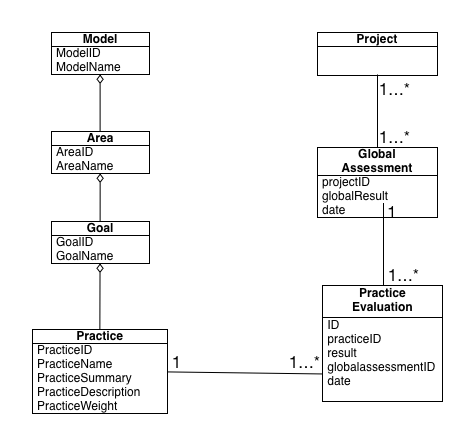
\includegraphics[width=0.8\textwidth]{ClassDiagram}
		\caption{Tables added to database}
		\label{fig:database}
	\end{center}
\end{figure}

\begin{figure}[h]
	\begin{center}
		\leavevmode
		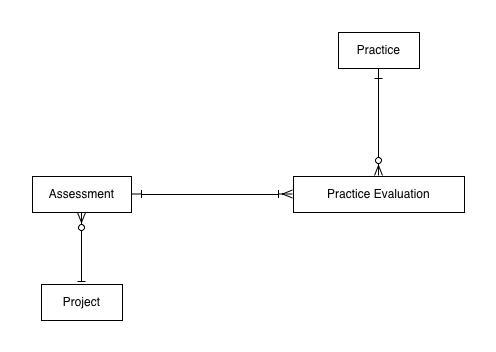
\includegraphics[width=0.6\textwidth]{Entity-Relationship-Model}
		\caption{Entity-relation}
		\label{fig:entity-relation}
	\end{center}
\end{figure}

\subsection{Module Structure}
Dar uma ideia, estrutura de criação - explicar o mvc de um modo da implementação
Facilidade de extensão e configuração - customização (mostrar como pode ser feito)

\begin{landscape}
\begin{figure}[h]
	\begin{center}
		\leavevmode
		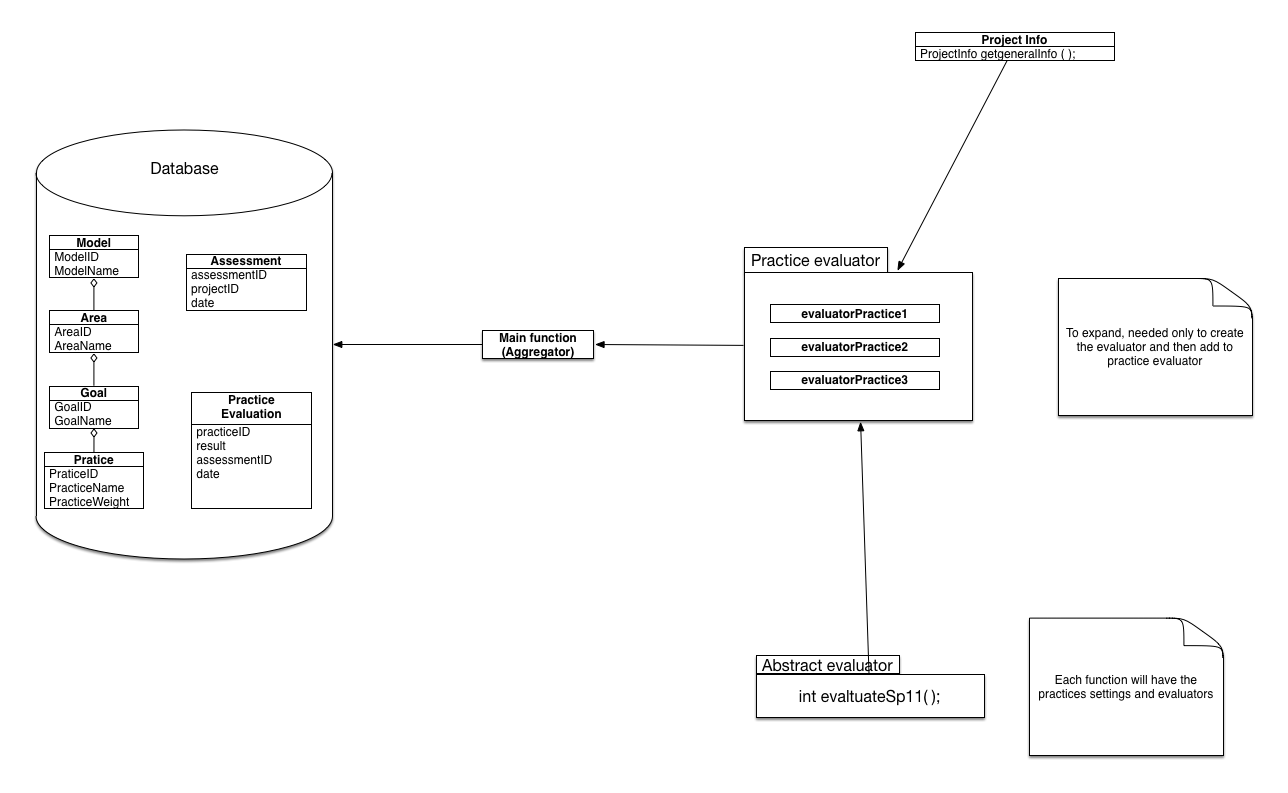
\includegraphics[width=1.2\textwidth]{esquema}
		\caption{Entity-relation}
		\label{fig:esquema}
	\end{center}
\end{figure}
\end{landscape}

\section{CMMI coverage} \label{sec:cmmicoverage}
Scraim extension to increase cmmi coverage

